% This document follows the topic-organised question collection in
% gadepall/cbse-papers/2015/math/12/main.tex. Obvious transcription errors are
% corrected in the question text where the intended statement is unambiguous.

\renewcommand{\theenumi}{\thesubsection.\arabic{enumi}}
\begin{enumerate}[label=\textbf{\thesubsection.\arabic*},leftmargin=4mm,itemsep=9pt]
\paragraph*{Vectors and three-dimensional geometry}
\item Find a vector of magnitude $\sqrt{171}$ perpendicular to both $\vec a=\myvec{1\\-2\\-3}$ and $\vec b=\myvec{3\\-1\\-2}$.
\solution Perpendicularity gives a homogeneous linear system for the unknown vector $\vec d=(d_1,d_2,d_3)^T$:
\[
M\vec d=0,\qquad
M=\begin{pmatrix}1&-2&-3\\3&-1&-2\end{pmatrix}.
\]
The two rows are independent, so $\operatorname{rank}(M)=2$ and rank--nullity gives $\dim\ker M=3-2=1$. Solving the two constraints gives the null-space basis
\[
\ker M=\operatorname{span}\{(1,-7,5)^T\}.
\]
Indeed, both row dot-products vanish. The basis vector has squared norm $1+49+25=75$. Scaling to magnitude $\sqrt{171}$ gives
\[
\vec d=\pm\frac{\sqrt{171}}{\sqrt{75}}(1,-7,5)^T
=\boxed{\pm\frac{\sqrt{57}}5(1,-7,5)^T}.
\]

\addtocounter{enumi}{3}
\item Let $\vec a=\myvec{1\\4\\2}$, $\vec b=\myvec{3\\-2\\7}$ and $\vec c=\myvec{2\\-1\\4}$. Find $\vec d$ perpendicular to both $\vec a,\vec b$ with $\vec c\cdot\vec d=27$.
\solution Use the antisymmetric bilinear vector operation, written as a determinant:
\[
\vec a\times\vec b=
\begin{vmatrix}
\hat i&\hat j&\hat k\\
1&4&2\\
3&-2&7
\end{vmatrix}
=(32,-1,-14)^T.
\]
The determinant changes sign when its two vector rows are interchanged, and its value is orthogonal to both input vectors. Since the common perpendicular space is one-dimensional, write $\vec d=t(32,-1,-14)^T$. The scalar constraint gives
\[
\vec c\cdot(\vec a\times\vec b)=2(32)+(-1)(-1)+4(-14)=9,
\qquad 9t=27.
\]
Thus $t=3$ and the corrected vector is
\[
\boxed{\vec d=(96,-3,-42)^T}.

\item Find the shortest distance between $\vec r=(1,2,3)+\lambda(2,3,4)$ and $\vec r=(2,4,5)+\mu(4,6,8)$.
\solution The two direction vectors are parallel, so the distance is the norm of the residual after projecting the point displacement onto their common direction. Let
\[
u=(2,3,4)^T,\qquad w=B-A=(1,2,2)^T.
\]
The orthogonal projector onto $\operatorname{span}\{u\}$ is
\[
P=u(u^Tu)^{-1}u^T=\frac1{29}
\begin{pmatrix}4&6&8\\6&9&12\\8&12&16\end{pmatrix}.
\]
The least-squares coefficient is $(u^Tu)^{-1}u^Tw=16/29$, and the perpendicular residual is
\[
r_\perp=(I-P)w=w-\frac{16}{29}u
=\frac1{29}(-3,10,-6)^T.
\]
Therefore
\[
d=\|r_\perp\|_2
=\frac{\sqrt{9+100+36}}{29}
=\boxed{\frac{\sqrt5}{\sqrt{29}}}.
\]
The residual is orthogonal to $u$, since $u^Tr_\perp=0$, which certifies that the projection is the closest point on the line.

\addtocounter{enumi}{3}
\item Find the plane through the intersection of $2x+y-z=3$ and $5x-3y+4z+9=0$ that is parallel to $\frac{x-1}{2}=\frac{y-3}{-4}=\frac{5-z}{-5}$.
\solution The intersection of the two given planes is a line, and every plane through that line belongs to the plane pencil
\[
\Pi_\lambda:\ (2x+y-z-3)+\lambda(5x-3y+4z+9)=0.
\]
Its normal vector is $n_\lambda=(2+5\lambda,1-3\lambda,-1+4\lambda)^T$. The specified parallel line has direction $d=(2,-4,5)^T$. A plane contains this direction exactly when its normal is orthogonal to it:
\[
d^Tn_\lambda=2(2+5\lambda)-4(1-3\lambda)+5(-1+4\lambda)=42\lambda-5=0.
\]
Hence $\lambda=5/42$. Substituting into the pencil and clearing the denominator gives the required affine plane:
\[
\boxed{109x+27y-22z-81=0}.

\addtocounter{enumi}{4}
\item Find where the line through $A(3,4,1)$ and $B(5,1,6)$ meets the plane through $P(2,1,2)$, $Q(3,1,0)$ and $R(4,-2,1)$.
\solution First obtain the plane as an affine constraint. Its two displacement vectors are
\[
Q-P=(1,0,-2)^T,\qquad R-P=(2,-3,-1)^T.
\]
A normal $n$ lies in the null space of the $2\times3$ matrix formed by these rows:
\[
\begin{pmatrix}1&0&-2\\2&-3&-1\end{pmatrix}n=0,
\qquad n\propto(2,1,1)^T.
\]
Thus the plane constraint is $2x+y+z=7$. The line parameterisation is
\[
(x,y,z)^T=(3,4,1)^T+t(2,-3,5)^T.
\]
Combining the line and plane equations produces the affine linear system
\[
\begin{pmatrix}
1&0&0&-2\\
0&1&0&3\\
0&0&1&-5\\
2&1&1&0
\end{pmatrix}
\begin{pmatrix}x\\y\\z\\t\end{pmatrix}
=
\begin{pmatrix}3\\4\\1\\7\end{pmatrix}.
\]
Its coefficient matrix is nonsingular, so the augmented system is consistent with a unique solution. Row reduction gives $t=-2/3$ and
\[
\boxed{(x,y,z)=\left(\frac53,6,-\frac73\right)}.

\addtocounter{enumi}{8}
\item Find the particular solution of $y'+y\tan x=3x^2+x^3\tan x$, given $y=0$ at $x=\pi/3$ and $x\ne\pi/2$.
\solution Set $u=y-x^3$. Substitution into the original equation cancels the known polynomial forcing:
\[
u'+u\tan x=0.
\]
Introduce the transformed independent variable $\tau=\ln(\sec x)$, for which $d\tau/dx=\tan x$. Away from $x=0$, the equation becomes the autonomous first-order system
\[
\frac{du}{d\tau}+u=0.
\]
At the initial point $x_0=\pi/3$, $\tau_0=\ln2$ and $u_0=-\pi^3/27$. We use unilateral Laplace transforms in a forward coordinate $\sigma=\tau-\tau_0\ge0$:
\[
\mathcal L\{u_\sigma\}=sU_+(s)-u_0,\qquad
(s+1)U_+(s)=u_0.
\]
Hence
\[
U_+(s)=-\frac{\pi^3}{27(s+1)},\qquad
u_+(\sigma)=-\frac{\pi^3}{27}e^{-\sigma}.
\]
For the side $0<x<\pi/3$, use the backward coordinate $\rho=\tau_0-\tau\ge0$. Then $du/d\rho-u=0$, and its unilateral transform gives
\[
(s-1)U_-(s)=u_0,\qquad
U_-(s)=-\frac{\pi^3}{27(s-1)},\qquad
u_-(\rho)=-\frac{\pi^3}{27}e^\rho.
\]
Since $e^{-\sigma}=e^\rho=2\cos x$ on the corresponding branches, both inverse transforms yield the same expression:
\[
u(x)=-\frac{2\pi^3}{27}\cos x,\qquad
\boxed{y(x)=x^3-\frac{2\pi^3}{27}\cos x}.
\]
The transformed coordinate has a turning point at $x=0$; the original equation is nonsingular there, so uniqueness extends this solution through $x=0$ to the full connected interval $-\pi/2<x<\pi/2$ containing the initial point. Direct substitution verifies the original ODE and $y(\pi/3)=0$.
\item If $y=\log\left(\frac{x}{a+bx}\right)^x$, prove that $x^3y''=(xy'-y)^2$.
\solution The logarithmic power is read as $y=\log\!\left[\left(\frac{x}{a+bx}\right)^x\right]=x\log\!\left(\frac{x}{a+bx}\right)$, on a domain where the logarithm is defined. Introduce the Euler differential operator $\theta=x\,d/dx$. For this $y$,
\[
\theta y- y=xy'-y=\frac{ax}{a+bx}.
\]
A second application of $\theta$ gives
\[
(\theta^2-\theta)y=x^2y'',\qquad
x(\theta^2-\theta)y=x^3y''.
\]
Directly evaluating this operator expression,
\[
x(\theta^2-\theta)y
=x\left(x^2y''\right)
=\frac{a^2x^2}{(a+bx)^2}
=(\theta y-y)^2.
\]
Therefore
\[
\boxed{x^3y''=(xy'-y)^2}.
\]

\addtocounter{enumi}{2}
\item If $A=\myvec{\cos\theta&\sin\theta\\\sin\theta&\cos\theta}$, find $\det(A^n)$ for natural $n$.
\solution The matrix is symmetric and has the orthonormal eigenvectors
\[
q_+=\frac1{\sqrt2}(1,1)^T,\qquad
q_-=\frac1{\sqrt2}(1,-1)^T.
\]
The corresponding eigenvalues are $\lambda_+=\cos\theta+\sin\theta$ and $\lambda_-=\cos\theta-\sin\theta$. With $Q=(q_+\ q_-)$,
\[
A=Q\begin{pmatrix}\lambda_+&0\\0&\lambda_-\end{pmatrix}Q^T,\qquad
A^n=Q\begin{pmatrix}\lambda_+^n&0\\0&\lambda_-^n\end{pmatrix}Q^T.
\]
Consequently the determinant is the product of the eigenvalues raised to $n$:
\[
\det(A^n)=(\lambda_+\lambda_-)^n
=(\cos^2\theta-\sin^2\theta)^n
=\boxed{(\cos2\theta)^n}.

\addtocounter{enumi}{1}
\item Find the inverse of $\myvec{0&1&2\\1&2&3\\3&1&0}$ using elementary row operations.
\solution Use exact LU factorisation with a row permutation because the leading entry of $A$ is zero. Let
\[
A=\begin{pmatrix}0&1&2\\1&2&3\\3&1&0\end{pmatrix},\qquad
P=\begin{pmatrix}0&0&1\\0&1&0\\1&0&0\end{pmatrix}.
\]
Then
\[
PA=LU,\quad
L=\begin{pmatrix}1&0&0\\1/3&1&0\\0&3/5&1\end{pmatrix},\quad
U=\begin{pmatrix}3&1&0\\0&5/3&3\\0&0&1/5\end{pmatrix}.
\]
For the inverse, solve $LUx=Pe_j$ for each coordinate vector $e_j$ by forward substitution through $L$ and back substitution through $U$. Collecting the three exact rational solutions is equivalent to
$A^{-1}=U^{-1}L^{-1}P$ and gives
\[
\boxed{
A^{-1}=
\begin{pmatrix}
3&-2&1\\
-9&6&-2\\
5&-3&1
\end{pmatrix}}.
\]
Indeed, multiplication verifies $AA^{-1}=I$.

\addtocounter{enumi}{5}
\item If $a+b+c\ne0$ and $\mydet{a&b&c\\b&c&a\\c&a&b}=0$, prove that $a=b=c$.
\solution Let $\omega=e^{2\pi i/3}$, so $1+\omega+\omega^2=0$ and $\omega^3=1$. The three-point DFT eigenvectors diagonalise this cyclic matrix:
\[
C=\begin{pmatrix}a&b&c\\b&c&a\\c&a&b\end{pmatrix},
\quad
\lambda_0=a+b+c,\quad
\lambda_1=a+b\omega+c\omega^2,\quad
\lambda_2=a+b\omega^2+c\omega.
\]
The determinant is the product of the DFT eigenvalues:
\[
0=\det C=\lambda_0\lambda_1\lambda_2.
\]
By assumption $\lambda_0=a+b+c\ne0$, so $\lambda_1\lambda_2=0$. Since $a,b,c$ are real, $\lambda_2=\overline{\lambda_1}$; hence $|\lambda_1|^2=0$ and $\lambda_1=0$. Its real and imaginary parts give
\[
a-\frac{b+c}{2}=0,\qquad \frac{\sqrt3}{2}(b-c)=0.
\]
Thus $b=c$ and $a=b$, proving
\[
\boxed{a=b=c}.

\item A trust receives Rs. 30,000 per month. Half is spent on care, and 2\% of the amount spent is collected from beneficiaries. The unspent balance is deposited in a bank. Find the monthly interest rate needed for total monthly income of Rs. 1800.
\solution Let $u$ be the monthly contribution collected from beneficiaries and $v$ the bank interest. Half of Rs. $30,000$ is spent, so
\[
u=0.02(15000)=300.
\]
The total monthly income is Rs. $1800$, so
\[
u+v=1800,\qquad u=300.
\]
Write this system as an augmented matrix:
\[
\left[\begin{array}{cc|c}1&1&1800\\1&0&300\end{array}\right]
\xrightarrow{R_2\leftarrow R_2-R_1}
\left[\begin{array}{cc|c}1&1&1800\\0&-1&-1500\end{array}\right]
\xrightarrow{R_2\leftarrow -R_2}
\left[\begin{array}{cc|c}1&1&1800\\0&1&1500\end{array}\right].
\]
Eliminate $v$ from the first row:
\[
R_1\leftarrow R_1-R_2:\qquad
\left[\begin{array}{cc|c}1&0&300\\0&1&1500\end{array}\right]\qquad\eqref{eq:gaussian-elimination}.
\]
Thus $u=300$ and $v=1500$. The deposit is Rs. $15000$, therefore
\[
r=\frac{1500}{15000}\times100\%=10\%\text{ per month}.
\]
\par\smallskip
\noindent\textbf{Code reference -}
\par\noindent\fbox{\parbox{\dimexpr\linewidth-2\fboxsep-2\fboxrule\relax}{\centering\texttt{codes/Q37.py}}}
\par\smallskip

\paragraph*{Integration and area}
\item Evaluate $\displaystyle I=\int_0^{\pi/2}\frac{\cos^2x}{1+3\sin^2x}\,dx$.
\solution Let $t=\tan x$. Then $dx=dt/(1+t^2)$ and the integral becomes
\[
I=\int_0^\infty\frac{dt}{(1+t^2)(1+4t^2)}=\int_0^\infty\left[-\frac1{3(1+t^2)}+\frac4{3(1+4t^2)}\right]dt.
\]
Evaluating the arctangent limits gives $I=-\pi/6+\pi/3=\pi/6\qquad\eqref{eq:scaled-arctan-integral-38},\ \eqref{eq:arctan-integral-38}$.

\item Evaluate $\displaystyle\int_0^{\pi/4}\frac{\sin x+\cos x}{3+\sin2x}\,dx$.
\solution Set $u=\sin x-\cos x$, so $du=(\sin x+\cos x)dx$ and $\sin2x=1-u^2$. The limits become $u=-1$ and $u=0$. Hence
\[
I=\int_{-1}^{0}\frac{du}{4-u^2}=\left[\frac14\ln\left|\frac{2+u}{2-u}\right|\right]_{-1}^{0}=\frac14\ln3\qquad\eqref{eq:int-rational-39}.
\]

\item Evaluate $\displaystyle\int\frac{\sin x-x\cos x}{x(x+\sin x)}\,dx$.
\solution Since
\[
\frac{d}{dx}\ln\left|\frac{x}{x+\sin x}\right|=\frac{\sin x-x\cos x}{x(x+\sin x)}\qquad\eqref{eq:log-derivative-40},
\]
the integral is $\ln\left|\frac{x}{x+\sin x}\right|+C$.

\item Evaluate $\displaystyle\int\frac{x^3}{(x-1)(x^2+1)}\,dx$.
\solution Polynomial division and partial fractions give
\[
\frac{x^3}{(x-1)(x^2+1)}=1+\frac1{2(x-1)}+\frac{x-1}{2(x^2+1)}\qquad\eqref{eq:partial-fractions-41}.
\]
Therefore
\[
x+\frac12\ln|x-1|+\frac14\ln(x^2+1)-\frac12\tan^{-1}x+C.
\]

\item Find $\displaystyle\int\frac{x\,dx}{1+x\tan x}$.
\solution Rewrite the integrand as $x\cos x/(\cos x+x\sin x)$. Since $d(\cos x+x\sin x)/dx=x\cos x$,
\[
\int\frac{x\,dx}{1+x\tan x}=\ln|\cos x+x\sin x|+C\qquad\eqref{eq:log-derivative-42}.
\]

\item Evaluate $\displaystyle\int\frac{x^4}{(x-1)(x^2+1)}\,dx$.
\solution Division gives $x^4/[(x-1)(x^2+1)]=x+1+1/[(x-1)(x^2+1)]$. Decompose the last term as
\[
\frac1{(x-1)(x^2+1)}=\frac1{2(x-1)}-\frac{x+1}{2(x^2+1)}\qquad\eqref{eq:partial-fractions-43}.
\]
Thus
\[
\frac{x^2}{2}+x+\frac12\ln|x-1|-\frac14\ln(x^2+1)-\frac12\tan^{-1}x+C.
\]

\item Evaluate $\displaystyle\int_0^{\pi/2}\frac{5\sin x+3\cos x}{\sin x+\cos x}\,dx$.
\solution Write the numerator as $4(\sin x+\cos x)+(\sin x-\cos x)$. Then
\[
I=4\int_0^{\pi/2}dx-\left[\ln(\sin x+\cos x)\right]_0^{\pi/2}=2\pi\qquad\eqref{eq:trig-split-44}.
\]

\item Find $\displaystyle\int\left[\log(\log x)+\frac1{(\log x)^2}\right]dx$.
\solution Differentiate $x\log(\log x)-x/\log x$ to check that it equals the integrand. Hence
\[
x\log(\log x)-\frac{x}{\log x}+C,\qquad x>1\text{ for a real-valued }\log(\log x).
\]

\item If the area bounded by $y^2=16ax$ and $y=4mx$ is $a^2/2$, find $m$.
\solution Use the upper branch $y=4\sqrt{ax}$. At an intersection with $y=4mx$,
\[
4\sqrt{ax}=4mx\quad\Longrightarrow\quad x=0\quad\text{or}\quad x=\frac{a}{m^2}.
\]
For positive slope, the area is the integral of the parabola minus the line:
\begin{align*}
A&=\int_0^{a/m^2}\left(4\sqrt{ax}-4mx\right)\,dx\\
 &=\left[\frac{8\sqrt a}{3}x^{3/2}-2mx^2\right]_0^{a/m^2}\\
 &=\frac{8a^2}{3m^3}-\frac{2a^2}{m^3}=\frac{2a^2}{3m^3}\qquad\eqref{eq:area-between-46}.
\end{align*}
Set the result equal to the given area:
\[
\frac{2a^2}{3m^3}=\frac{a^2}{2}\quad\Longrightarrow\quad4=3m^3\quad\Longrightarrow\quad m=\sqrt[3]{\frac43}.
\]
The graph uses $a=1$ for visibility; the value of $m$ is independent of that scale.
\begin{figure}[H]\centering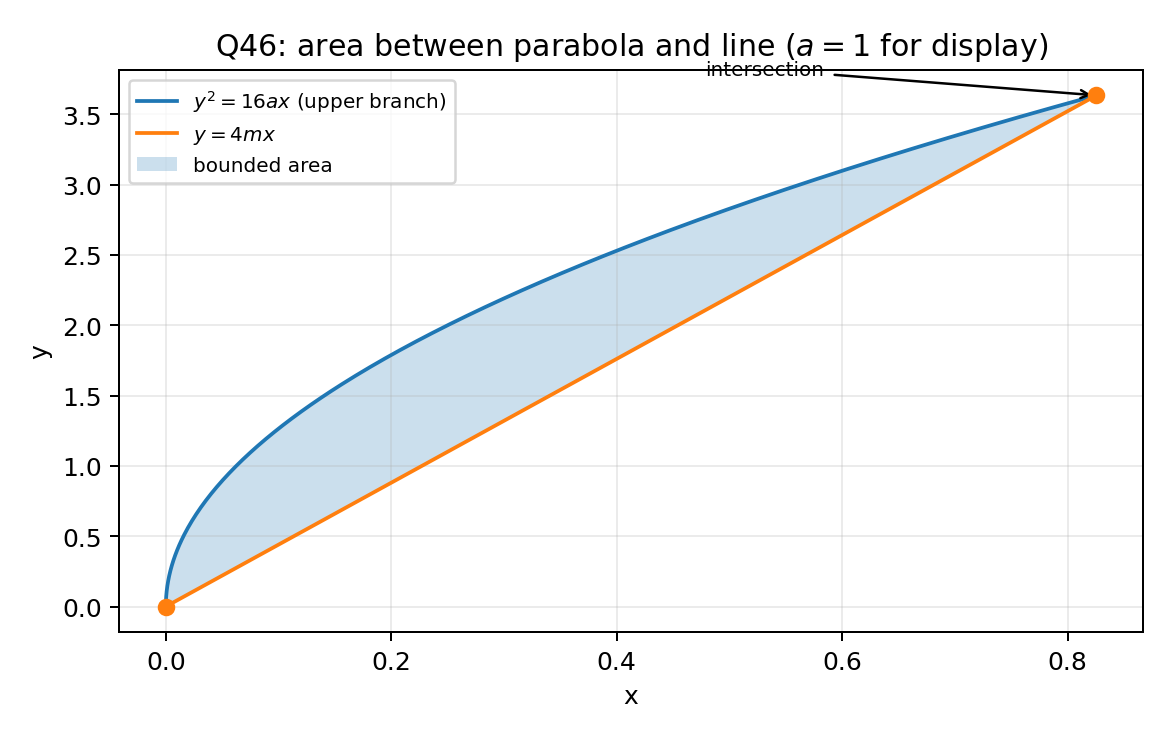
\includegraphics[width=0.92\linewidth]{figs/Q46_ParabolaArea.png}\end{figure}
\par\smallskip
\noindent\textbf{Code reference -}
\par\noindent\fbox{\parbox{\dimexpr\linewidth-2\fboxsep-2\fboxrule\relax}{\centering\texttt{codes/Q46.py}}}
\par\smallskip

\item Find the area of $\{(x,y):x^2+y^2\le4,\;x+y\ge2\}$ by integration.
\solution The chord $x+y=2$ meets the circle at $(0,2)$ and $(2,0)$. For $0\le x\le2$, the upper circle boundary is $y=\sqrt{4-x^2}$ and the line is $y=2-x$. Therefore
\begin{align*}
A&=\int_0^2\left(\sqrt{4-x^2}-(2-x)\right)dx\\
 &=\underbrace{\int_0^2\sqrt{4-x^2}\,dx}_{\text{quarter-circle area }=\pi}
 -\underbrace{\int_0^2(2-x)\,dx}_{\text{triangle area }=2}\\
 &=\pi-2\quad\text{square units}\qquad\eqref{eq:area-between-47}.
\end{align*}
The graph shades the circular segment above the chord.
\begin{figure}[H]\centering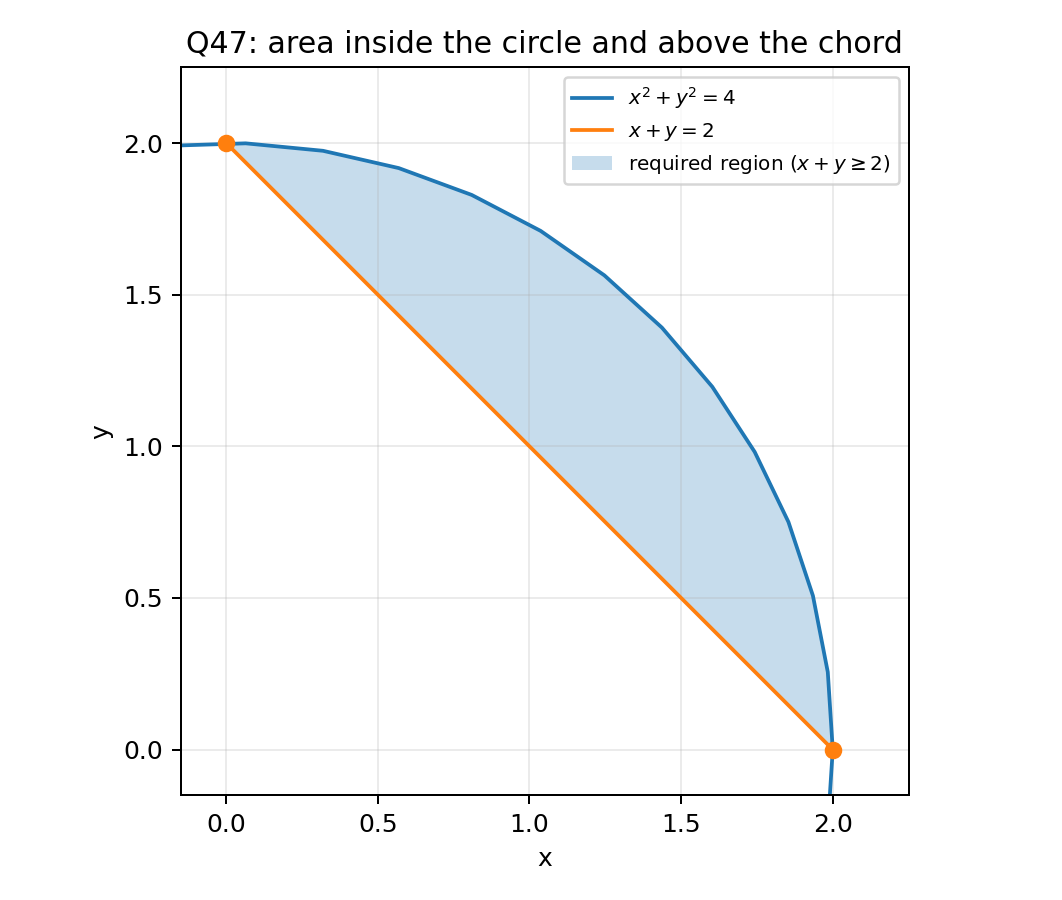
\includegraphics[width=0.92\linewidth]{figs/Q47_CircleSegment.png}\end{figure}
\par\smallskip
\noindent\textbf{Code reference -}
\par\noindent\fbox{\parbox{\dimexpr\linewidth-2\fboxsep-2\fboxrule\relax}{\centering\texttt{codes/Q47.py}}}
\par\smallskip

\paragraph*{Functions and relations}
\item Discuss continuity and differentiability of $f(x)=|x|+|x-1|$ on $(-1,2)$.
\solution Interpret $f$ as a piecewise-linear static characteristic. With $r^+=\max(r,0)$,
\[
f(x)=1+2(-x)^++2(x-1)^+.
\]
Resolving the two switching points gives
\[
f(x)=
\begin{cases}
1-2x,&-1<x<0,\\
1,&0\le x<1,\\
2x-1,&1\le x<2.
\end{cases}
\]
At $x=0$ and $x=1$, the adjacent branches agree and equal $1$; thus the characteristic is continuous on $(-1,2)$.

On each smooth segment, the incremental gain is constant:
\[
f'(x)=
\begin{cases}
-2,&-1<x<0,\\
0,&0<x<1,\\
2,&1<x<2.
\end{cases}
\]
At the switching points the one-sided gains disagree:
\[
f'_-(0)=-2\ne0=f'_+(0),\qquad
f'_-(1)=0\ne2=f'_+(1).
\]
The classical derivative therefore fails exactly at $0$ and $1$. The slope is nondecreasing across the breakpoints, so the characteristic is convex. Its Clarke generalized derivatives are
\[
\partial_C f(0)=[-2,0],\qquad \partial_C f(1)=[0,2].
\]
Since every segment has slope magnitude at most $2$, the complete piecewise characteristic is globally Lipschitz with the sharp constant
\[
|f(x_2)-f(x_1)|\le2|x_2-x_1|,\qquad x_1,x_2\in(-1,2).
\]
Thus it is continuous and bounded on the stated interval, but nonsmooth at the two switching points.
\item On $\mathbb R$, define $(a,b)\in R$ when $a-b+\sqrt3$ is irrational. Determine whether $R$ is reflexive, symmetric and transitive.
\solution We test each property separately using the criteria in \eqref{eq:relation-properties-49}.

\textbf{1. Reflexive.} Reflexivity requires $(a,a)\in R$ for every real $a$. Substituting $b=a$ gives
\[
a-a+\sqrt3=\sqrt3,
\]
which is irrational. Therefore $R$ is reflexive.

\textbf{2. Symmetric.} Symmetry requires $(a,b)\in R$ to imply $(b,a)\in R$. Choose $a=\sqrt3$ and $b=0$. Then
\[
a-b+\sqrt3=2\sqrt3
\]
is irrational, so $(a,b)\in R$. Reversing the pair gives
\[
b-a+\sqrt3=0,
\]
which is rational, so $(b,a)\notin R$. Hence $R$ is not symmetric.

\textbf{3. Transitive.} Transitivity requires $(a,b),(b,c)\in R$ to imply $(a,c)\in R$. Choose $a=\sqrt3$, $b=0$, and $c=2\sqrt3$. Then
\[
a-b+\sqrt3=2\sqrt3,\qquad b-c+\sqrt3=-\sqrt3,
\]
both irrational, so $(a,b),(b,c)\in R$. However,
\[
a-c+\sqrt3=\sqrt3-2\sqrt3+\sqrt3=0,
\]
which is rational. Thus $(a,c)\notin R$, and $R$ is not transitive.

\textbf{Conclusion.} $R\text{ is reflexive, but neither symmetric nor transitive.}$

\item On $\mathbb R\times\mathbb R$, define $(a,b)*(c,d)=(a+c,b+d)$. Prove commutativity and associativity, and find the identity and the inverse of $(3,-5)$.
\solution The set $\mathbb R^2$ is closed under componentwise addition. For any $u,v,w\in\mathbb R^2$, real-number addition gives
\[
u*v=v*u,\qquad (u*v)*w=u*(v*w),
\]
so the operation is commutative and associative. The identity is $e=(0,0)$ because $u*e=e*u=u$. For each $(a,b)$, the inverse is $(-a,-b)$, since
\[
(a,b)*(-a,-b)=(0,0).
\]
In particular, $(3,-5)^{-1}=(-3,5)$. These facts establish that $(\mathbb R^2,*)$ is an Abelian group.

\item On $\{0,1,2,3,4,5,6\}$ define $a*b=a+b$ if $a+b<7$, and $a*b=a+b-7$ otherwise. Give the operation table and show that 0 is the identity and $7-a$ is the inverse for nonzero $a$.
\solution This is addition in the cyclic group $\mathbb Z_7$, with operation $a*b=(a+b)\bmod7$. Its table is
\[
\begin{array}{c|rrrrrrr}
* &0&1&2&3&4&5&6\\\hline
0&0&1&2&3&4&5&6\\
1&1&2&3&4&5&6&0\\
2&2&3&4&5&6&0&1\\
3&3&4&5&6&0&1&2\\
4&4&5&6&0&1&2&3\\
5&5&6&0&1&2&3&4\\
6&6&0&1&2&3&4&5
\end{array}
\]
Closure follows from reduction modulo 7, and associativity follows from associativity of integer addition before reduction. The operation is commutative. Row and column 0 show that 0 is the identity. Each nonzero $a$ has inverse $7-a$, because $a+(7-a)\equiv0\pmod7$. Since 7 is prime, every nonzero residue generates the whole group; in particular, $1$ is a generator and the group is cyclic of order 7.

\item Find any point of discontinuity of $f(x)=x-|x-x^2|$, $x\in[-1,1]$.
\solution Treat the expression as a piecewise nonlinear static transfer characteristic. Since $x-x^2=x(1-x)$ is nonpositive on $[-1,0]$ and nonnegative on $[0,1]$,
\[
f(x)=
\begin{cases}
2x-x^2,&-1\le x\le0,\\
x^2,&0\le x\le1.
\end{cases}
\]
The two branches both give 0 at $x=0$, so the left and right limits agree with $f(0)$; the endpoint values are also the corresponding one-sided limits. Therefore there are no discontinuities on $[-1,1]$.

The incremental gains on the open pieces are
\[
f'_-(x)=2-2x\in(2,4),\qquad f'_+(x)=2x\in(0,2).
\]
At the switching point, the one-sided derivatives are $f'_-(0)=2$ and $f'_+(0)=0$, so the characteristic is continuous but not classically differentiable at 0. The derivative magnitude is bounded by 4 throughout the interval, hence the characteristic is globally Lipschitz with sharp constant $L=4$:
\[
|f(x)-f(y)|\le4|x-y|,\qquad x,y\in[-1,1].
\]
The range is $[-3,1]$, so the response is bounded. There is no discontinuity, but there is a corner at the switching point.

\item A man steps forward with probability $0.4$ and backward with probability $0.6$. Find the probability that after 5 steps he is one step away from his starting point.
\solution Encode a forward step as exponent $+1$ and a backward step as exponent $-1$. The one-step bilateral $Z$-transform (Laurent probability-generating function) is
\[
G_1(z)=0.4z+0.6z^{-1}.
\]
Independence and convolution of step displacements imply
\[
G_5(z)=G_1(z)^5
=(0.4z+0.6z^{-1})^5
=\sum_{k=0}^5\binom5k(0.4)^k(0.6)^{5-k}z^{2k-5}.
\]
The displacement probabilities are the Laurent coefficients. In particular,
\[
P(D=1)=[z^1]G_5(z)=\binom53(0.4)^3(0.6)^2=0.2304,
\]
\[
P(D=-1)=[z^{-1}]G_5(z)=\binom52(0.4)^2(0.6)^3=0.3456.
\]
The events are disjoint, so the required probability is
\[
\boxed{P(|D|=1)=0.2304+0.3456=0.576}.
\]
The characteristic function is obtained by restricting the Laurent variable to the unit circle, $z=e^{i\omega}$:
\[
\varphi_D(\omega)=G_5(e^{i\omega})
=(0.4e^{i\omega}+0.6e^{-i\omega})^5.
\]

\item A girl throws a die. If it shows 1 or 2, she tosses a coin three times; otherwise she tosses it once. Given that exactly one tail was obtained, find the probability that the die showed 3, 4, 5 or 6.
\solution Let $A$ be the hypothesis that the die shows 1 or 2, and $B$ the hypothesis that it shows 3, 4, 5 or 6. Let $E$ be the observation of exactly one tail. The prior odds are
\[
\frac{P(B)}{P(A)}=\frac{4/6}{2/6}=2.
\]
The likelihoods are
\[
P(E\mid A)=\binom31(1/2)^3=\frac38,\qquad
P(E\mid B)=\frac12.
\]
Thus the likelihood ratio in favour of $B$ is
\[
\Lambda=\frac{P(E\mid B)}{P(E\mid A)}
=\frac{1/2}{3/8}=\frac43.
\]
Bayes' odds form multiplies prior odds by the likelihood ratio:
\[
\frac{P(B\mid E)}{P(A\mid E)}
=\frac{P(B)}{P(A)}\Lambda
=2\cdot\frac43=\frac83.
\]
Normalising the posterior odds gives
\[
\boxed{P(B\mid E)=\frac{8}{8+3}=\frac8{11}}.

\item An urn contains 5 red and 2 black balls. Two balls are drawn without replacement. Let $X$ be the number of black balls. State its possible values and find its mean and variance.
\solution The without-replacement count has hypergeometric probability-generating function
\[
G_X(s)=\sum_{k=0}^{2}
\frac{\binom2k\binom5{2-k}}{\binom72}s^k
=\frac{10+10s+s^2}{21}.
\]
Its coefficients give $P(X=0)=10/21$, $P(X=1)=10/21$, and $P(X=2)=1/21$. Differentiating the PGF,
\[
E[X]=G'_X(1)=\frac{12}{21}=\frac47,\qquad
E[X(X-1)]=G''_X(1)=\frac2{21}.
\]
Therefore $E[X^2]=G''_X(1)+G'_X(1)=2/3$ and
\[
\boxed{\operatorname{Var}(X)=\frac23-\left(\frac47\right)^2=\frac{50}{147}}.
\]
To expose the without-replacement dependence, let $I_1,I_2$ indicate black on draw 1 and draw 2. Then
\[
\operatorname{Cov}(I_1,I_2)=P(I_1=I_2=1)-P(I_1=1)P(I_2=1)
=\frac1{21}-\frac4{49}=-\frac5{147}<0.
\]
The negative covariance is the dependence created by removing a ball after the first draw.

\item In 3 trials of a binomial distribution, the probability of exactly 2 successes is 9 times the probability of 3 successes. Find the success probability.
\solution The binomial probability-generating polynomial is
\[
B(z)=(1-p+pz)^3.
\]
Its coefficients are $P(X=2)=3p^2(1-p)$ and $P(X=3)=p^3$. The stated equality gives
\[
3p^2(1-p)=9p^3
\quad\Longleftrightarrow\quad
3p^2(1-4p)=0.
\]
The admissible interval is $0\le p\le1$. The boundary value $p=0$ is valid: both probabilities are zero and the stated equality $0=9\cdot0$ holds. The non-degenerate root is $p=1/4$. Hence the complete solution set is
\[
\boxed{p=0\quad\text{or}\quad p=\frac14}.
\]

\item An urn contains 3 red and 5 black balls. A ball is drawn, its colour recorded and returned, and 2 more balls of that colour are added. Then two balls are drawn without replacement. Find the probability both are red.
\solution Treat the reinforced composition as a stochastic state transition. The initial state is $S_0=(3,5)$. The first draw and reinforcement produce one of two states:
\[
(3,5)\xrightarrow[\;P=3/8\;]{R}(5,5),\qquad
(3,5)\xrightarrow[\;P=5/8\;]{B}(3,7).
\]
From state $(5,5)$, the two subsequent draws are red without replacement with probability
\[
P(RR\mid S_R)=\frac5{10}\frac4{9}=\frac29.
\]
From state $(3,7)$, that probability is
\[
P(RR\mid S_B)=\frac3{10}\frac2{9}=\frac1{15}.
\]
The transition tree therefore gives
\[
P(RR)=\frac38\frac29+\frac58\frac1{15}
=\boxed{\frac18}.
\]
The branch probabilities sum to one and the urn state is updated before the two-draw terminal transition.

\addtocounter{enumi}{1}
\item Solve graphically: minimise $z=3x+5y$ subject to $x+2y\ge10$, $x+y\ge6$, $3x+y\ge8$, $x,y\ge0$.
\solution The primal linear programme is
\[
\min\ 3x+5y\quad\text{subject to}\quad
Ax\ge b,\quad x\ge0,
\]
where $A=\begin{pmatrix}1&2\\1&1\\3&1\end{pmatrix}$, $b=(10,6,8)^T$. Its dual is
\[
\max\ 10u_1+6u_2+8u_3
\quad\text{subject to}\quad
u_1+u_2+3u_3\le3,\quad
2u_1+u_2+u_3\le5,\quad u\ge0.
\]
The feasible primal point $(x,y)=(2,4)$ has objective 26 and satisfies the first two primal constraints with equality; the third has slack 2. The dual point $u=(2,1,0)$ is feasible and has objective $20+6=26$. Weak duality bounds every primal objective below by every dual feasible value. Since the feasible values agree, strong duality certifies
\[
\boxed{x=2,\quad y=4,\quad z_{\min}=26}.
\]
Complementary slackness also holds: $u_1,u_2>0$ correspond to tight primal constraints, $u_3=0$ corresponds to the slack third constraint, and both positive primal variables force their dual constraints to be tight.

\item A dealer has Rs. 57,600 and space for at most 20 sewing machines. An electronic machine costs Rs. 3600 and earns Rs. 220 profit; a manual machine costs Rs. 2400 and earns Rs. 180 profit. How should he invest to maximise profit?
\solution Let $x,y$ be the numbers of electronic and manual machines. The primal programme is
\[
\max\ 220x+180y,\quad
3x+2y\le48,\quad x+y\le20,\quad x,y\ge0.
\]
Its dual is
\[
\min\ 48u+20v,\quad
3u+v\ge220,\quad2u+v\ge180,\quad u,v\ge0.
\]
At the intersection of the two primal resource limits, $(x,y)=(8,12)$ and the profit is Rs. 3920. Since both primal variables are positive, complementary slackness requires both dual inequalities to bind:
\[
3u+v=220,\qquad2u+v=180,
\]
which gives $(u,v)=(40,100)$. This dual point is feasible and its objective is
\[
48(40)+20(100)=3920.
\]
The primal feasible plan and dual feasible certificate have equal objectives, so weak/strong duality proves global optimality:
\[
\boxed{8\text{ electronic and }12\text{ manual machines; maximum profit Rs. }3920}.
\]
Both primal resource constraints are tight, consistent with $u,v>0$.

\addtocounter{enumi}{3}
\item A tangent to $x^2+y^2=4$ at a point in the first quadrant meets the positive axes at $A$ and $B$. Find the minimum of $OA+OB$.
\solution Parameterise the point of tangency by $(u,v)$ with $u,v>0$ and $u^2+v^2=4$. The tangent line is $uX+vY=4$, so its positive intercepts are $OA=4/u$ and $OB=4/v$. The constrained nonlinear problem is
\[
\min_{u,v>0}F(u,v)=\frac4u+\frac4v
\quad\text{subject to}\quad g(u,v)=u^2+v^2-4=0.
\]
The KKT stationarity conditions for an interior optimum are
\[
-\frac4{u^2}+2\lambda u=0,\qquad
-\frac4{v^2}+2\lambda v=0.
\]
Eliminating $\lambda$ gives $u^3=v^3$, hence $u=v=\sqrt2$. The objective is
\[
F_{\min}=\frac4{\sqrt2}+\frac4{\sqrt2}=\boxed{4\sqrt2}.
\]
As either $u\downarrow0$ or $v\downarrow0$, the objective tends to infinity; the feasible first-quadrant arc is otherwise compact. Therefore this unique stationary point is the global minimum.

\item Find the maximum area of an isosceles triangle inscribed in $\frac{x^2}{16}+\frac{y^2}{9}=1$ with its vertex at an end of the major axis.
\solution Fix the major-axis vertex at $(4,0)$ and use symmetry for the other vertices $(u,v)$ and $(u,-v)$, with $-4\le u\le4$ and $v=3\sqrt{1-u^2/16}$. The area objective and feasibility constraint are
\[
A(u,v)=v(4-u),\qquad
h(u,v)=\frac{u^2}{16}+\frac{v^2}{9}-1=0,\quad v\ge0.
\]
For an interior maximiser, the Lagrangian $\mathcal L=v(4-u)-\lambda h(u,v)$ yields
\[
-v=\lambda\frac{u}{8},\qquad
4-u=\lambda\frac{2v}{9}.
\]
Eliminating $\lambda$ gives $u^2-2u-8=0$, so $u=4$ or $u=-2$. The candidate $u=4$ is a degenerate zero-area boundary. At $u=-2$, $v=3\sqrt3/2$ and
\[
A= (4-(-2))\frac{3\sqrt3}{2}
=\boxed{9\sqrt3}.
\]
The other endpoint $u=-4$ gives $A=0$, while the endpoint $u=4$ also gives zero. Hence the feasible stationary candidate at $u=-2$ is the global maximum.

